\documentclass[11pt,a4paper]{article}

\usepackage[T1]{fontenc}
\usepackage[utf8]{inputenc}
\usepackage{lmodern}
\usepackage[margin=3.5cm]{geometry}
\usepackage{xcolor}
\usepackage{graphicx}
\usepackage{amsmath}
\usepackage[most]{tcolorbox}
\usepackage{titlesec}
\usepackage{fancyhdr}
\usepackage[hidelinks]{hyperref}

\graphicspath{{../}{./}}

\definecolor{headingblue}{HTML}{1A3A5C}
\definecolor{boxcream}{HTML}{F4F1E7}
\definecolor{boxbar}{HTML}{8C6D2F}
\definecolor{rulegold}{HTML}{A08B5B}
\definecolor{pagegrey}{HTML}{808080}

\titleformat{\section}{\normalfont\large\bfseries\color{headingblue}}
  {}{0pt}{}
\titlespacing*{\section}{0pt}{1.6\baselineskip}{0.6\baselineskip}

\pagestyle{fancy}
\fancyhf{}
\renewcommand{\headrulewidth}{0pt}
\fancyfoot[C]{\color{pagegrey}\small\thepage}

\newtcolorbox{keybox}{
  enhanced, breakable, colback=boxcream, colframe=boxcream,
  boxrule=0pt, leftrule=3pt, colbacktitle=boxcream,
  borderline west={3pt}{0pt}{boxbar},
  left=10pt, right=10pt, top=8pt, bottom=8pt,
  sharp corners
}

\setlength{\parindent}{0pt}
\setlength{\parskip}{0.7\baselineskip}

\begin{document}

\begin{center}
  {\LARGE\bfseries\color{headingblue} Sharper, or taller?}\\[6pt]
  {\large Two ways a wave can become infinite, and how to tell them apart}\\[12pt]
  {\normalsize Munawar Kazmi \quad$\bullet$\quad munawarkazmi.com}\\[6pt]
  {\normalsize A plain-language guide to \textbf{degregorio-blowup}, an open
  study of how simplified models of fluid flow tear themselves apart.}\\[4pt]
  {\normalsize Code, data, and every figure:
  github.com/munawarkazmi/degregorio-blowup}
\end{center}

\vspace{4pt}
{\color{rulegold}\hrule height 0.8pt}
\vspace{10pt}

\section{A wave, a circle, and two forces}

Take a wave running around a circle. Not water exactly, but the mathematical
skeleton of one: a number at every point saying how fast the fluid is spinning
there.

Two things act on it at once, and they want opposite outcomes.

The first is \textbf{stretching}. Spinning fluid pulls on itself. Where the
wave is already steep, the pulling makes it steeper, and a steeper wave pulls
harder still. Left alone, this feeds back on itself so violently that the wave
becomes infinitely tall in a finite amount of time. Not eventually. By a
particular Tuesday.

The second is \textbf{transport}. The fluid is also moving, and it carries the
wave along with it. This is a calming influence, because it slides the sharp
part of the wave away from the place that is doing the sharpening.

Whether a fluid can tear itself apart in finite time is one of the Clay
Millennium Prize problems, and nobody can answer it for real fluids in three
dimensions. So people study small models that keep the fight between these two
forces and throw away everything else. This is a study of one such model.

\section{The dial}

The model has a dial on it, a number written $a$, which sets how much transport
there is. Turn it to zero and transport is switched off entirely. Turn it to
one and transport is at full strength.

Both ends of the dial are completely understood, and that is what makes the
model worth using.

At $a = 0$, with no transport at all, the whole thing was solved by hand in
1985. Starting from a simple wave, it becomes infinite at time 2. Exactly 2.
You can write the answer on a napkin.

At $a = 1$, with transport at full strength, something remarkable happens.
There is a particular wave shape for which the two forces cancel each other
exactly, at every point, forever. Drop that wave in and it simply sits there.
It never sharpens and it never fades.

\begin{keybox}
Everything interesting is between the two ends of the dial. At one end the
answer is known and violent. At the other it is known and perfectly still.
Nobody can solve what happens in between, so it has to be computed.
\end{keybox}

\section{What was built}

A program that follows the wave forward in time, and a set of checks on whether
it can be believed.

The checks matter more than the program. There are 19 of them, and each one
compares the program against something already known with certainty: the exact
1985 answer, the wave that should sit still, quantities that must not change,
convergence rates that theory predicts in advance. One of them predicts an
error should shrink by a factor of 16 when a setting is halved, and the
measured factors are 16.65, 16.28, 16.16 and 16.07.

None of this proves the program is right. It means that everywhere the answer
was already known, the program found it, which is the most that can be asked of
an instrument.

\section{Two ways to become infinite}

Turn the dial part way, run the model, and the wave becomes infinite. That much
happens for every setting below one. The blowup time stretches out as the dial
approaches one, from 2 to about 57, but it always arrives.

What was not expected is that it arrives in two completely different ways.

\begin{figure}[htbp]
  \centering
  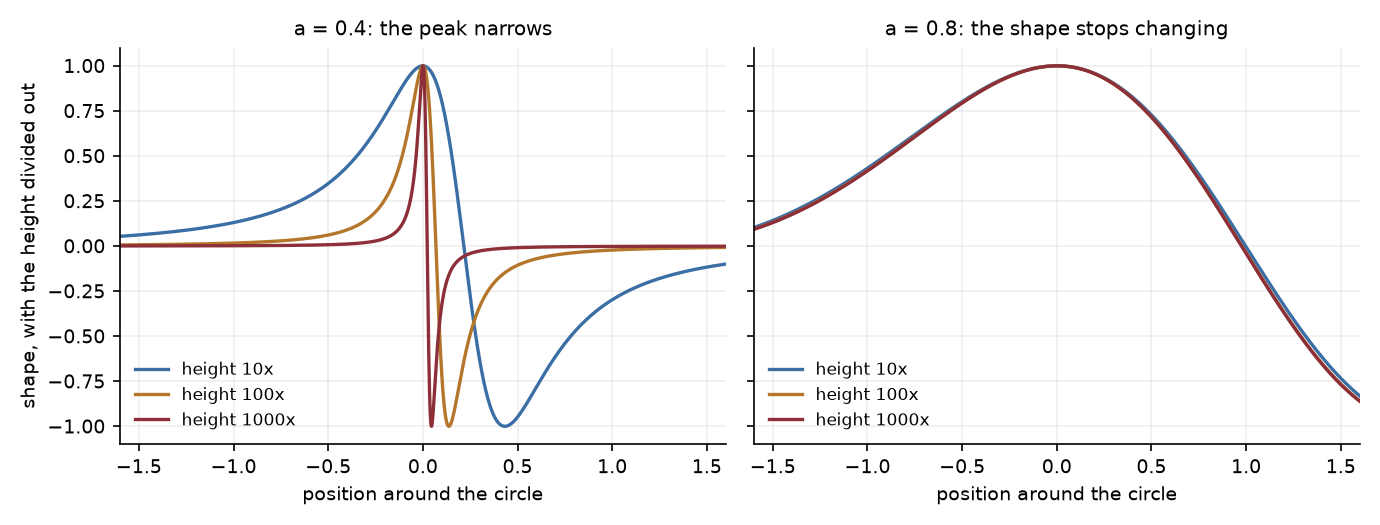
\includegraphics[width=\textwidth]{fig_two_regimes.png}
  \caption{The same wave at three moments, when its height has grown ten,
  a hundred and a thousand times over. Each snapshot has been divided by its
  own height, so the growth is removed and only the shape is left. On the left
  the shape keeps changing. On the right it has stopped.}
\end{figure}

With the dial low, the peak gets \textbf{narrower} as it gets taller. It
concentrates into an ever thinner spike. This is the intuitive picture of
something blowing up, and it is what the 1985 solution does.

With the dial high, around 0.8, something stranger happens. The peak gets
taller and its shape does not change at all. It is the same curve throughout,
scaled up. Divide out the height and the snapshots lie on top of one another to
seven decimal places.

\begin{keybox}
Two different infinities. In one the wave becomes a needle. In the other it
keeps its shape exactly and simply grows without limit, like a photograph
enlarged over and over.
\end{keybox}

\section{The shape that stops changing}

The second kind is the useful one, because a shape that stops changing can be
solved for directly.

Instead of running a simulation and watching numbers get large, you can ask:
what curve has the property that the two forces reshape it into a scaled copy
of itself? That is an equation with a fixed answer, and it can be solved on a
laptop in seconds, to twelve decimal places, with nothing running away.

There is a good way to check whether the curve found this way is really the one
the fluid finds. The equation fixes not just the shape but its exact height,
and that height can also be measured from a simulation, in a completely
separate way, by watching how fast the peak grows. The two numbers share
nothing except the setting of the dial.

They agree to five decimal places.

The same curve turns up from every starting wave tried: sixteen random ones, a
whole family of shifted ones, several built by hand. All of them, to seven
digits. It is not an artefact of where you start.

\section{A number you can write down}

Here is the part that was least expected.

The curve is singular somewhere. There is a point on it where the mathematics
stops being smooth, and everything about the blowup, including how rough the
final shape is, is governed by what happens there.

That point turns out to be where the fluid's own velocity is zero. A stagnation
point: the one place the flow is not going anywhere.

And at that point, one quantity can be worked out exactly, in three lines of
algebra, with no computation at all. If the dial is set to $a$, that quantity
is
\[
  \frac{1}{1 - a}.
\]
Set the dial to 0.8 and it is 5. Not approximately 5. The simulation agrees to
fourteen decimal places.

\begin{keybox}
In a problem where almost nothing closes in exact form, one number does, and it
falls out of a calculation short enough to do on the back of an envelope.
\end{keybox}

There is a second quantity at a second stagnation point, and it governs the
roughness. That one refused to close. It was computed to five digits, every
simple formula for it was tested and rejected, and the honest conclusion is
that it is set by the problem as a whole rather than by anything local. If it
had a tidy form, this model would probably not be hard.

\section{The kink}

How rough is the final shape?

Smooth enough to draw without lifting the pen, and smooth enough that its slope
never jumps. But go one level further, to the rate at which the slope changes,
and there is a jump: from $-2.27$ on one side of that stagnation point to
$+2.27$ on the other.

You could not see this by eye. The curve looks perfectly ordinary. It is the
kind of defect that only appears when you ask the third question about it.

It also settles a small puzzle. Other researchers have proved that in this
family the blowup shapes are smooth. The shape here is not, and both statements
are correct. Their work is on an infinite line; this is on a circle. On a
circle the velocity is forced to be zero somewhere, so a stagnation point must
exist, and the roughness has nowhere else to go.

\section{When the instrument caught itself}

Most of the wrong turns in this project came from the same mistake, and it is
worth naming because it is so ordinary.

Repeatedly, a curve that was gently bending got a straight line drawn through
it, the fit looked excellent, and the answer was wrong. A measure of fit
quality of 0.99 out of 1 accompanied a conclusion that later had to be
withdrawn. Four separate numbers were produced this way and four were retracted.

One case is a fair summary of the rest. A roughness exponent was measured at
3.045, which is suspiciously close to 3, so it was worth asking whether it was
exactly 3. It is not. But the 3.045 was wrong too. The measurement window
straddled two regions that were biased in opposite directions, and the true
value, 3.0024, was sitting inside the data the whole time behind a badly chosen
window.

There was also a moment where an exact identity was derived, tested, and
apparently disproved by its own test, before the disproof turned out to be a
rounding error caused by subtracting two enormous numbers.

\begin{keybox}
All of these are still in the repository, with the retractions written next to
the claims they retract. A wrong answer you can reproduce is worth more than a
right one you cannot.
\end{keybox}

\section{What this does not show}

None of this is a proof. It is careful computation with the checks written
down, and that is a different thing. A genuine proof in this area requires
certified arithmetic that tracks its own error bars, which has not been done
here.

The behaviour as the dial approaches one, which is the case that most resembles
the real problem, is not resolved. The blowup time grows, but at what rate
could not be determined: the measured exponent wanders between 0.64 and 0.82
instead of settling. What was established is why that is hard rather than
merely unfinished, which is a smaller result but a real one.

There is also an open set of starting waves, discovered by accident, that never
blow up at all and instead fade away. What organises them is not understood.

Finally, all of this is one small model in one dimension. The three-dimensional
question it stands in for remains exactly as open as it was.

\section{Why it matters}

The Millennium problem asks whether a fluid can become infinitely violent from
a perfectly ordinary start. Nobody can settle it directly, so the working
strategy across the field is to build up technique on small models that keep
the essential fight and discard the geometry.

This is one of those models, and the useful finding is not a number. It is that
the blowup here has a fixed shape which can be computed directly rather than
chased, that the shape is stable so the fluid actually finds it, and that one
of the constants describing it can be written down exactly.

Those are the properties a computer-assisted proof would need to work with.
Having them stated, measured, and checkable is the point.

\vspace{6pt}
{\color{rulegold}\hrule height 0.6pt}
\vspace{6pt}

{\small Every figure, every number, and the code that produced them are public,
along with a technical paper and a written record of the results that were
withdrawn.\\
Repository: github.com/munawarkazmi/degregorio-blowup}

\end{document}
